\documentclass[12pt]{article}

\usepackage{answers}
\usepackage{setspace}
\usepackage{graphicx}
\usepackage{enumitem}
\usepackage{multicol}
\usepackage{mathrsfs}
\usepackage[margin=1in]{geometry} 
\usepackage{amsmath,amsthm,amssymb}
\usepackage[english]{babel}

\newcommand{\N}{\mathbb{N}}
\newcommand{\Z}{\mathbb{Z}}
\newcommand{\C}{\mathbb{C}}
\newcommand{\R}{\mathbb{R}}

\DeclareMathOperator{\sech}{sech}
\DeclareMathOperator{\csch}{csch}

\newenvironment{theorem}[2][Theorem]{\begin{trivlist}
		\item[\hskip \labelsep {\bfseries #1}\hskip \labelsep {\bfseries #2.}]}{\end{trivlist}}
\newenvironment{definition}[2][Definition]{\begin{trivlist}
		\item[\hskip \labelsep {\bfseries #1}\hskip \labelsep {\bfseries #2.}]}{\end{trivlist}}
\newenvironment{proposition}[2][Proposition]{\begin{trivlist}
		\item[\hskip \labelsep {\bfseries #1}\hskip \labelsep {\bfseries #2.}]}{\end{trivlist}}
\newenvironment{lemma}[2][Lemma]{\begin{trivlist}
		\item[\hskip \labelsep {\bfseries #1}\hskip \labelsep {\bfseries #2.}]}{\end{trivlist}}
\newenvironment{exercise}[2][Exercise]{\begin{trivlist}
		\item[\hskip \labelsep {\bfseries #1}\hskip \labelsep {\bfseries #2.}]}{\end{trivlist}}
\newenvironment{solution}[2][Solution]{\begin{trivlist}
		\item[\hskip \labelsep {\bfseries #1}]}{\end{trivlist}}
\newenvironment{problem}[2][Problem]{\begin{trivlist}
		\item[\hskip \labelsep {\bfseries #1}\hskip \labelsep {\bfseries #2.}]}{\end{trivlist}}
\newenvironment{question}[2][Question]{\begin{trivlist}
		\item[\hskip \labelsep {\bfseries #1}\hskip \labelsep {\bfseries #2.}]}{\end{trivlist}}
\newenvironment{corollary}[2][Corollary]{\begin{trivlist}
		\item[\hskip \labelsep {\bfseries #1}\hskip \labelsep {\bfseries #2.}]}{\end{trivlist}}

\begin{document}
	
	% --------------------------------------------------------------
	%                         Start here
	% --------------------------------------------------------------
	
	\title{IT-Security}
	\author{Michael Gabler}
	
	\maketitle
	\tableofcontents
	\newpage
	
	\section{Definitions}
	
	\textbf{C-I-A Triad}
	\begin{enumerate}
		\item \textbf{C}onfidentiality: prevents unauthorized access to private data
		\item \textbf{I}ntegrity: protects information from being modified by unauthorized parties
		\item \textbf{A}vailability: authorized parties have access to the information when needed
		\item \textbf{A}uthenticity: Being able to verify a party
		\item \textbf{A}ccountability: To guaranty that a property or action belongs to one specific entity
	\end{enumerate}
	\textbf{Secrecy} Keep data hidden from unintended receivers\\
	\textbf{Privacy} Keep data about a person secret\\
	\textbf{Anonymity} Keep identity of a communicating party secret\\
	\textbf{Authorization} Allowing another entity to perform an action (access control)\\
	\textbf{Security Threat} A potential for violation of security (interruption (a), interception (p), modification (a), fabrication (a) of information) $\rightarrow$ splits up into active and passive\\
	\textbf{Security Attack} Action that compromises the security of information\\
	\textbf{Passive Attacker} Listens to communication and tries to gain information about it\\
	\textbf{Active Attacker} Manipulates communication (replay, alter, delete messages), Brute-force\\
	\textbf{Security Mechanism} A process or device that is designed to detect, prevent or recover from a security attack\\
	\textbf{Security Service} Service to prevent security attacks by implementing one or more mechanisms\\
	\textbf{Co-prime} are two numbers $a$ and $b$ when $\gcd(a,b) = 1$
	
	\section{One Key Cryptography}
	\textbf{Kerckhoffs' principle} \textit{The enemy knows the system} $\rightarrow$ The cipher should remain secure if the adversary knows the specification of the cipher\\
	$\Rightarrow$ not respecting this principle means \textbf{security by obscurity}\\
	\textbf{Encryption Scheme} is a pair of encryption ($Enc$) and decryption ($Dec$) algorithm with $Dec_k(Enc_k(m)) = m$ for every plaintext message $m \in M$ plaintext space and key $k \in K$ key space. $Dec_k(m) = c$ generates the cipher $c \in C$ ciphertext space.\\
	\textbf{Security of an encryption scheme} The adversary should not learn any additional information about $m$ when receiving $c$
	
	\subsection{Historical ciphers}
	\paragraph{Caesar's shift cipher} $M = {A,...,Z} = {0,...,25}$ words over alphabet\\
	$K = {0,...25}$\\
	$Enc_k(m_0,...,m_n) = (k+m_0 mod 26,..., k+m_n mod 26)$\\
	$Dec_k(c_0,...,c_n) = (c_0-k mod 26,..., c_n-k mod 26)$\\
	$\Rightarrow$ can be broken by brute force attack (try every key) since $|K| = 26$
	\paragraph{Substitution cipher}
	Do not shift each letter with the same key but use a mapping table\\
	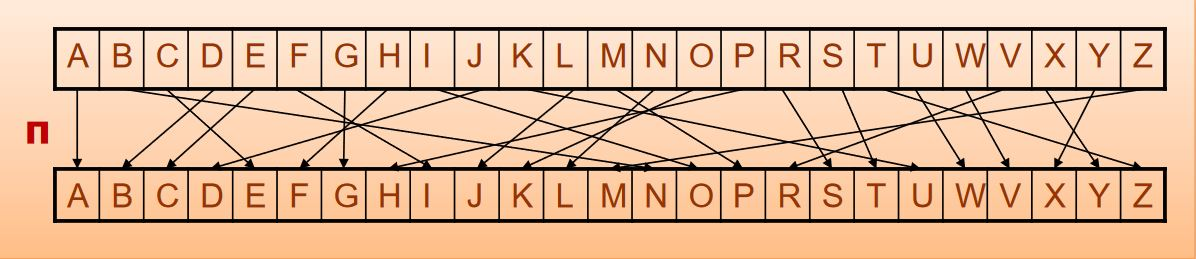
\includegraphics[width=\textwidth]{figures/substitution-cipher.JPG}\\
	$\Rightarrow$ can be broken by using statistical patterns: for example the letter E is the most frequent in the german language
	\paragraph{Vigenère cipher} Use a key with arbitrary length of letters. Each letter of the key defines the shift value for a plaintext letter. If the plaintext is longer than the key it must be repeated.\\
	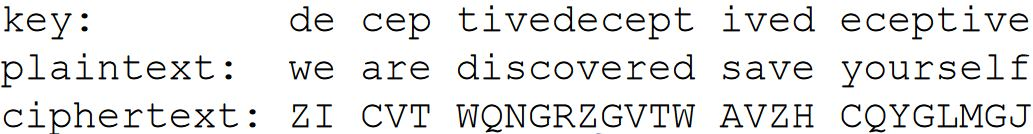
\includegraphics[width=\textwidth]{figures/vigenere-cipher.JPG}\\
	$\Rightarrow$ when the key is repeated its possible that the same letters are encrypted with the same shift which result in the same ciphertext. If such \textbf{identical parts} are found the \textbf{length of $k$} can be computed. Now it's possible to break the cipher by applying $|k|$-times the \textbf{frequency attack} from the substitution cipher.
	
	\subsection{One-time pad}
	$K = M = C = {0,1}^t$\\
	$Enc_k(m) = k xor m$\\
	$Dec_k(m) = k xor c$\\
	$\Rightarrow$ This is perfectly secure but not practical because a key can only be used once (otherwise same ciphertext for same plaintext) and therefore must be as long as the message which is also not practical. So there's no other perfectly secret cipher.\\
	$\Rightarrow$ Other encryption schemes rely on a limitation of the adversary's power (mostly meant \underline{computational} power)
	\textbf{Computational security} A system $X$ is $(t,\epsilon)$-secure if every Turing Machine that operates in time $t$ can break it with probability at most $\epsilon$ where $\epsilon$ is negligible (close to 0).
	
	\subsection{Attacks}
	\textbf{Ciphertext-only attack} The adversary has no information about the plaintext\\
	\textbf{Known plaintext attack} The plaintext is drawn from some distribution that the adversary does not control\\
	\textbf{Chosen-plaintext attack} The adversary can choose arbitrary plaintext and receives the ciphertext from it\\
	\textbf{Chosen-ciphertext attack} The adversary gets information by receiving the decryption of chosen ciphertexts
	
	\subsection{Modern cryptography}
	\textbf{One-way functions} are functions that are poly-time computable and hard to invert. Rely on a mathematical hardness assumption.\\
	\textbf{Pseudorandom generators (PRG)} Generate bits that look random. Depens on a seed (for example system time). Can be constructed by using a one-way function. They are cryptographic if it's not % TODO finish definition\\
	\textbf{Stream cipher} cipher with an infinite stream of bits as output (for example RC4 used for WEP, WPA) $\rightarrow$ PRGs are stream ciphers\\
	\textbf{Block ciphers} are almost equal to pseudorandom permutations (PRP) (permutation is pseudorandom if it can't be distinguished from a real random permutation). Block ciphers permute a predefined amount of plaintext or data into a ciphertext of the same length. Popular block ciphers are:\\
	\begin{tabular}{|l|c|c|}
		\hline 
		& \textbf{key length} & \textbf{block length} \\ 
		\hline 
		DES (Data Encryption Standard) & 56 & 64 \\ 
		\hline 
		IDEA (International Data Encryption Algorithm) & 128 & 64 \\ 
		\hline 
		AES (Advanced Encryption Standard) & 128, 192 or 256 & 128 \\ 
		\hline 
	\end{tabular}\\
	\textbf{Padding} If a stream encrypted with a block cipher the last plaintext block needs to be padded (for example PKCS\#5: add $x$ bytes with value $x$)
	
	\subsubsection{Modes of operation}
	They describe how large amounts of plaintext can be encrypted using block ciphers.\\
	\begin{tabular}{|l|c|c|c|c|}
		\hline 
		& ECB & CBC & OFB & CTR \\ 
		\hline 
		error in $c_i$ affects & $c_i$ & $c_i$, $c_{i+1}$ & $c_i$ & $c_i$ \\ 
		\hline 
		parallel encryption & yes & no & no & yes \\ 
		\hline 
		parallel decryption & yes & yes & no & yes \\ 
		\hline 
		change 1 bit of $m_i$ & $c_i$ & all & $c_i$ & $c_i$ \\ 
		\hline 
	\end{tabular}

	\paragraph{Electronic Codebook (ECB)} $\leftarrow$ not secure\\
	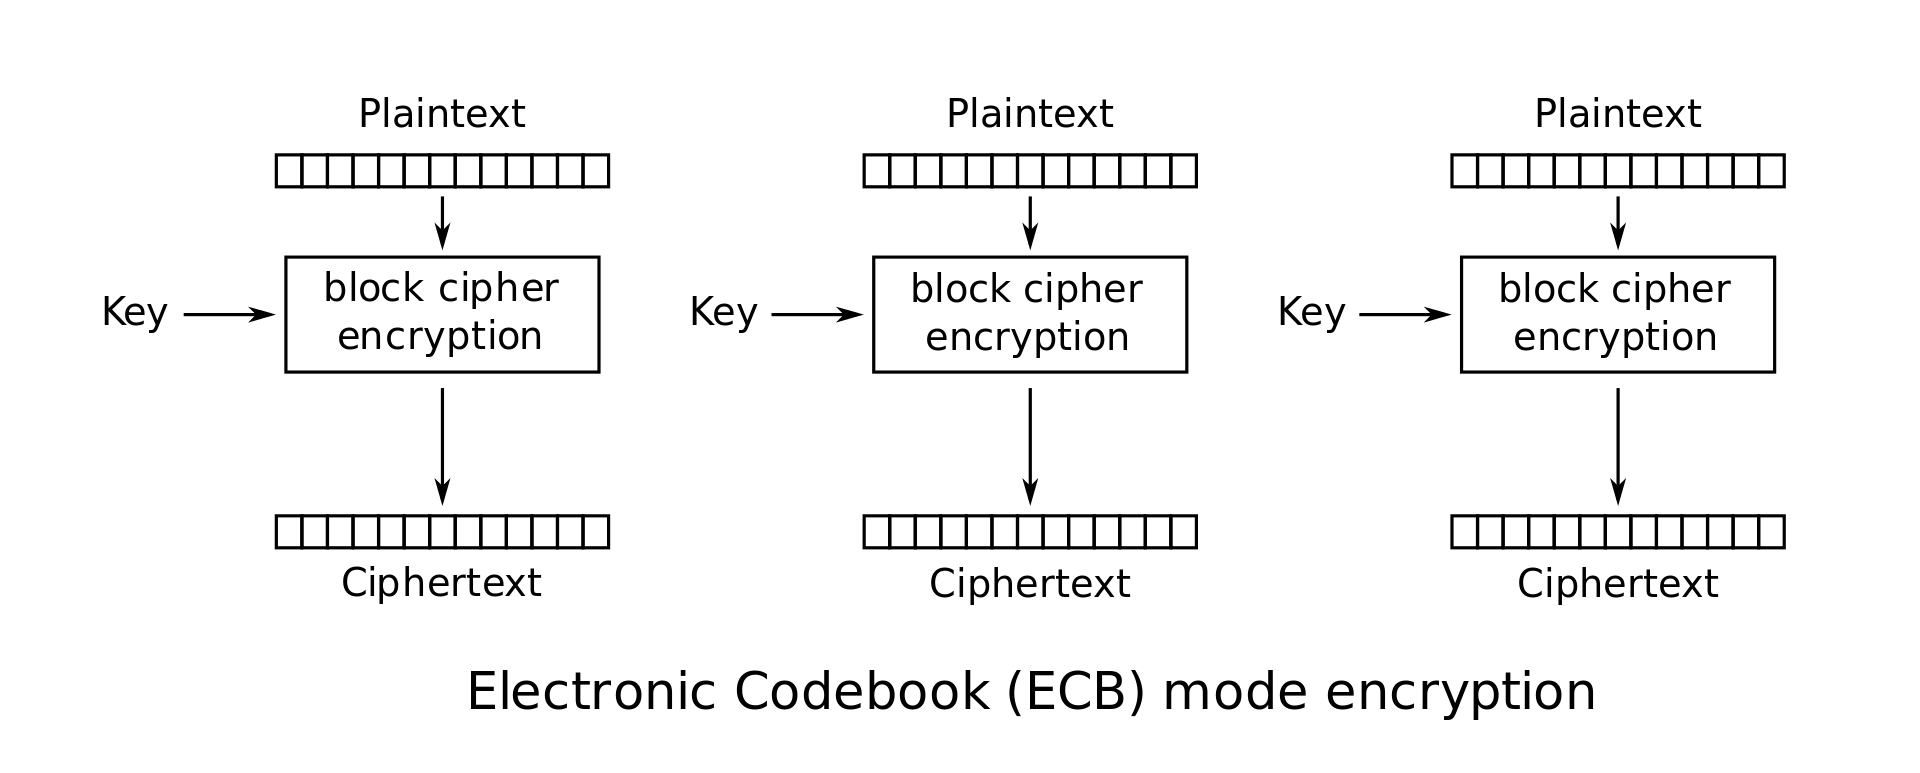
\includegraphics[width=0.5\textwidth]{figures/Ecb_encryption.png}
	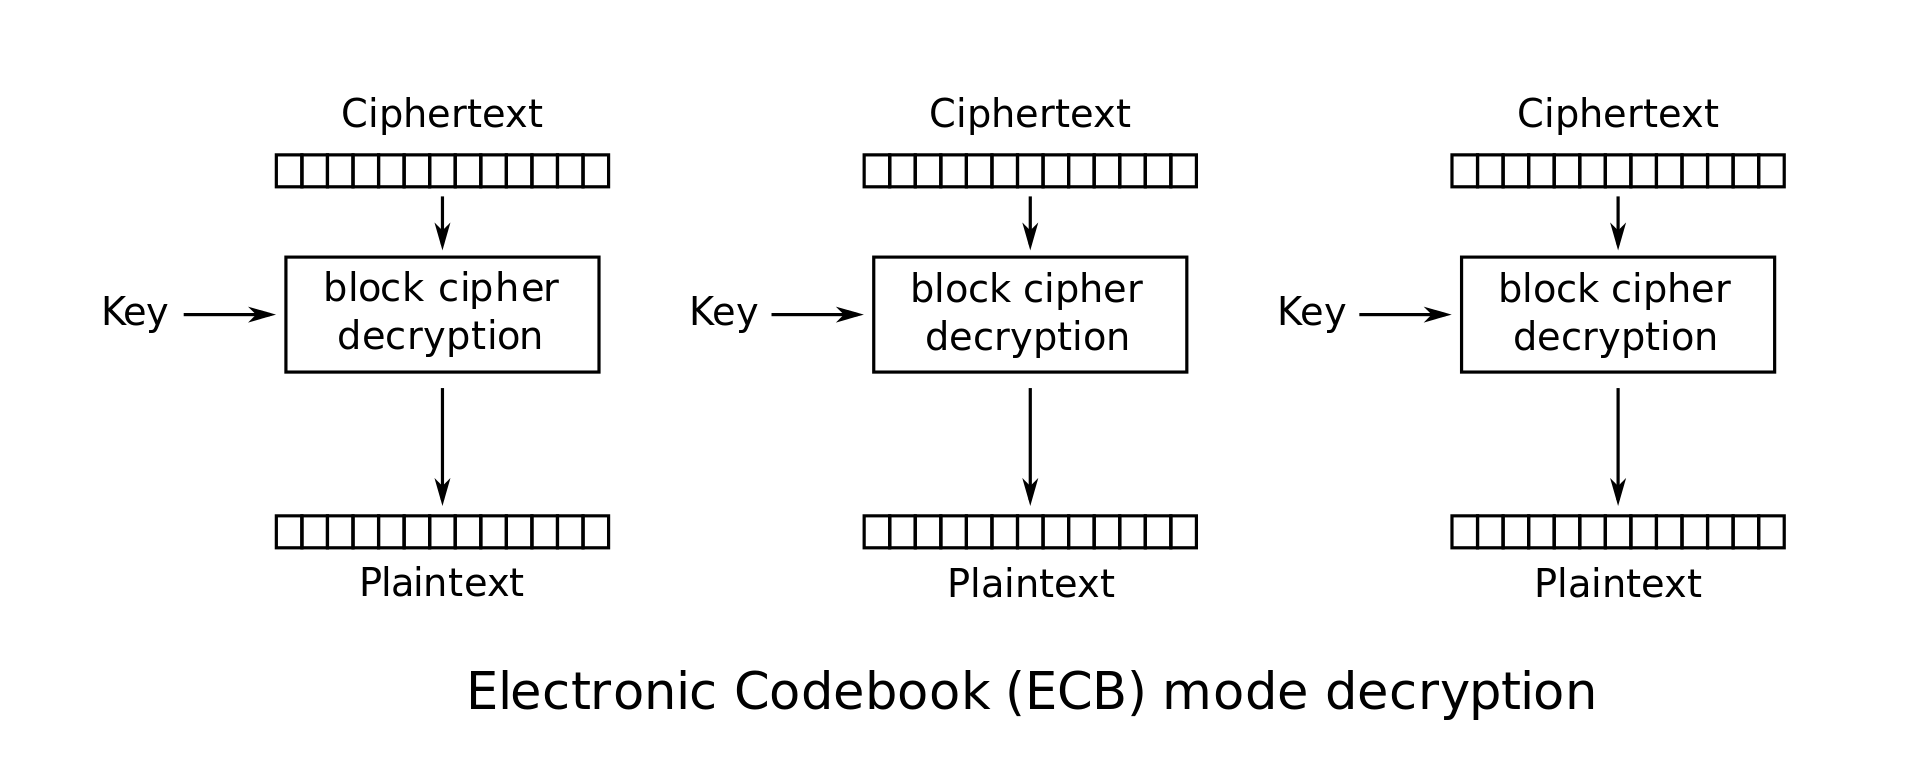
\includegraphics[width=0.5\textwidth]{figures/Ecb_decryption.png}\\
	$\Rightarrow$ the same plaintext block will result the same ciphertext block
	\paragraph{Cipher-Block Chaining (CBC)} .\\
	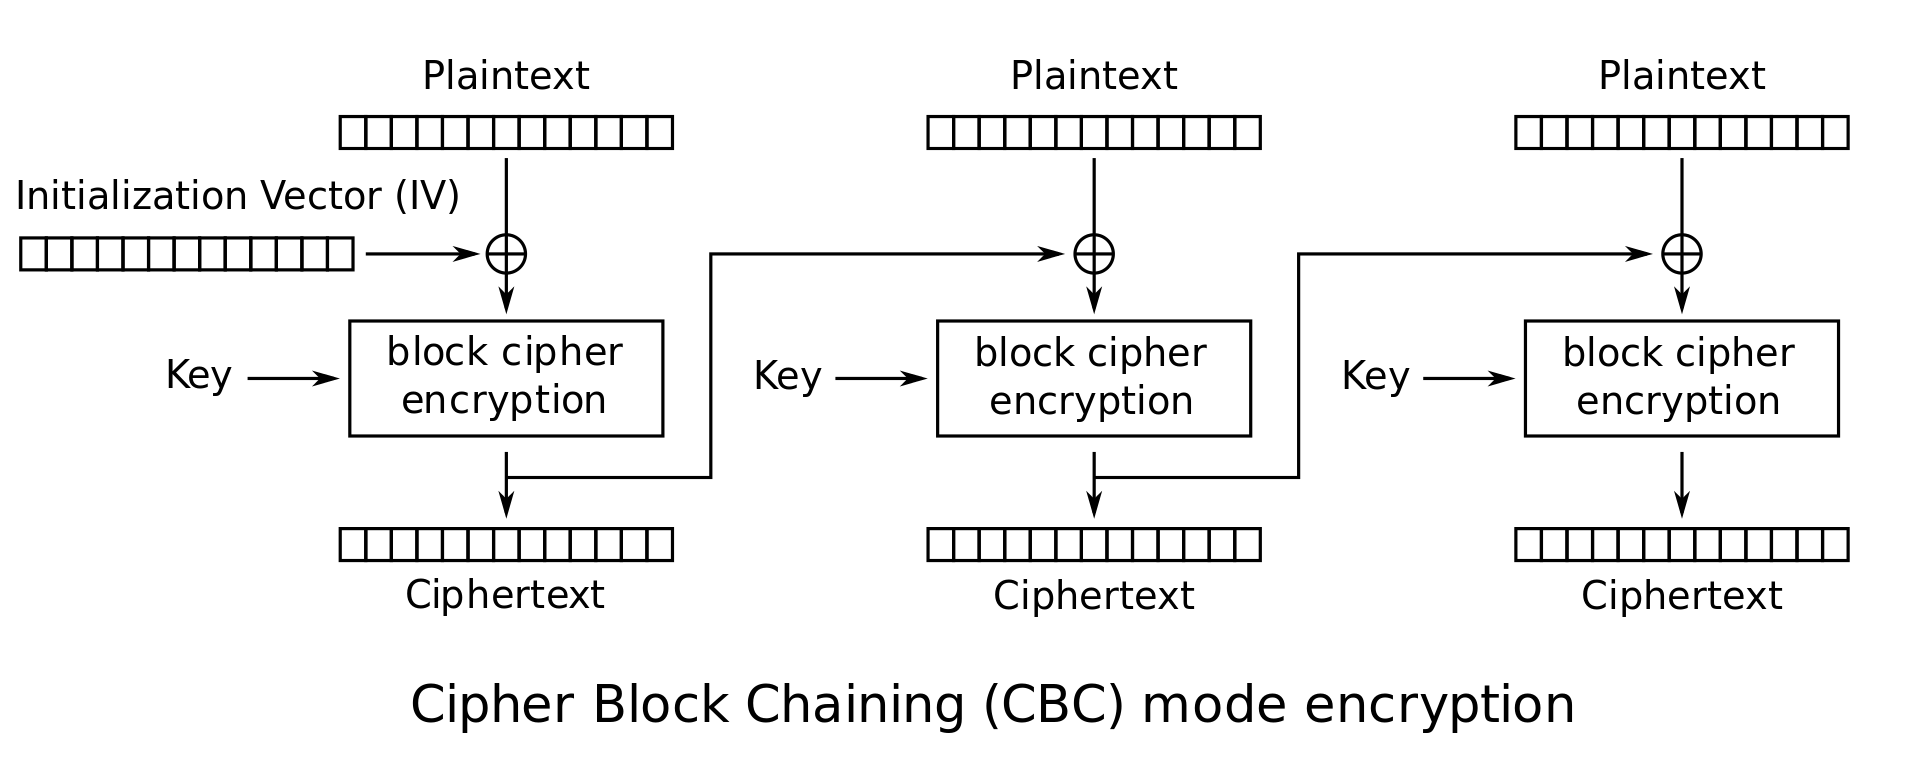
\includegraphics[width=0.5\textwidth]{figures/Cbc_encryption.png}
	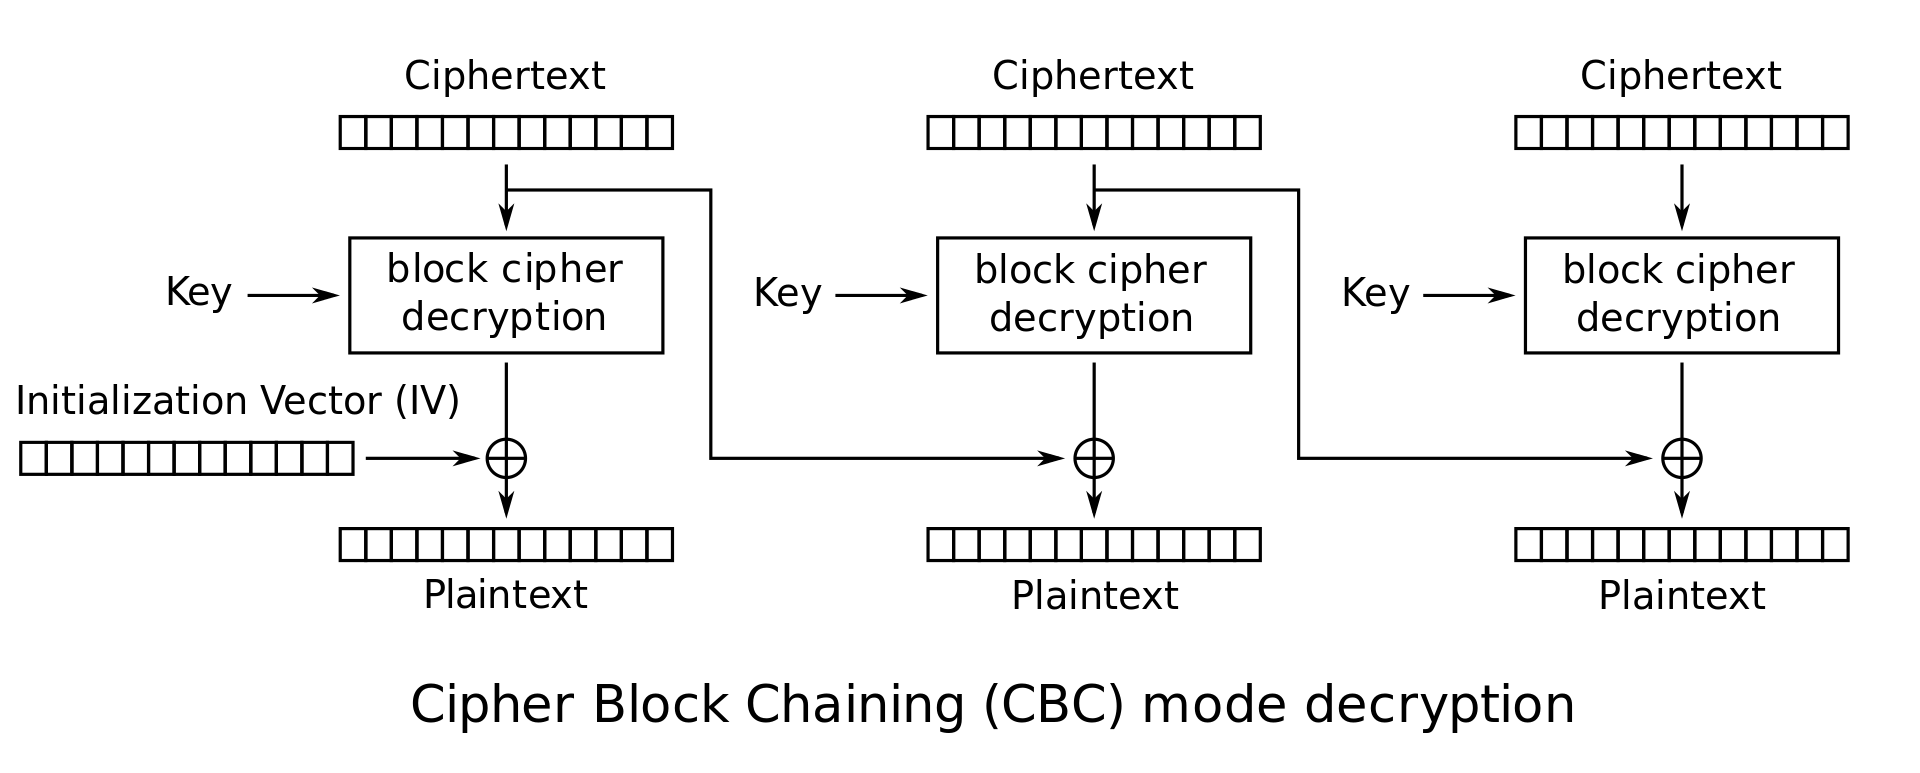
\includegraphics[width=0.5\textwidth]{figures/Cbc_decryption.png}
	\paragraph{Output Feedback Mode (OFB)} .\\
	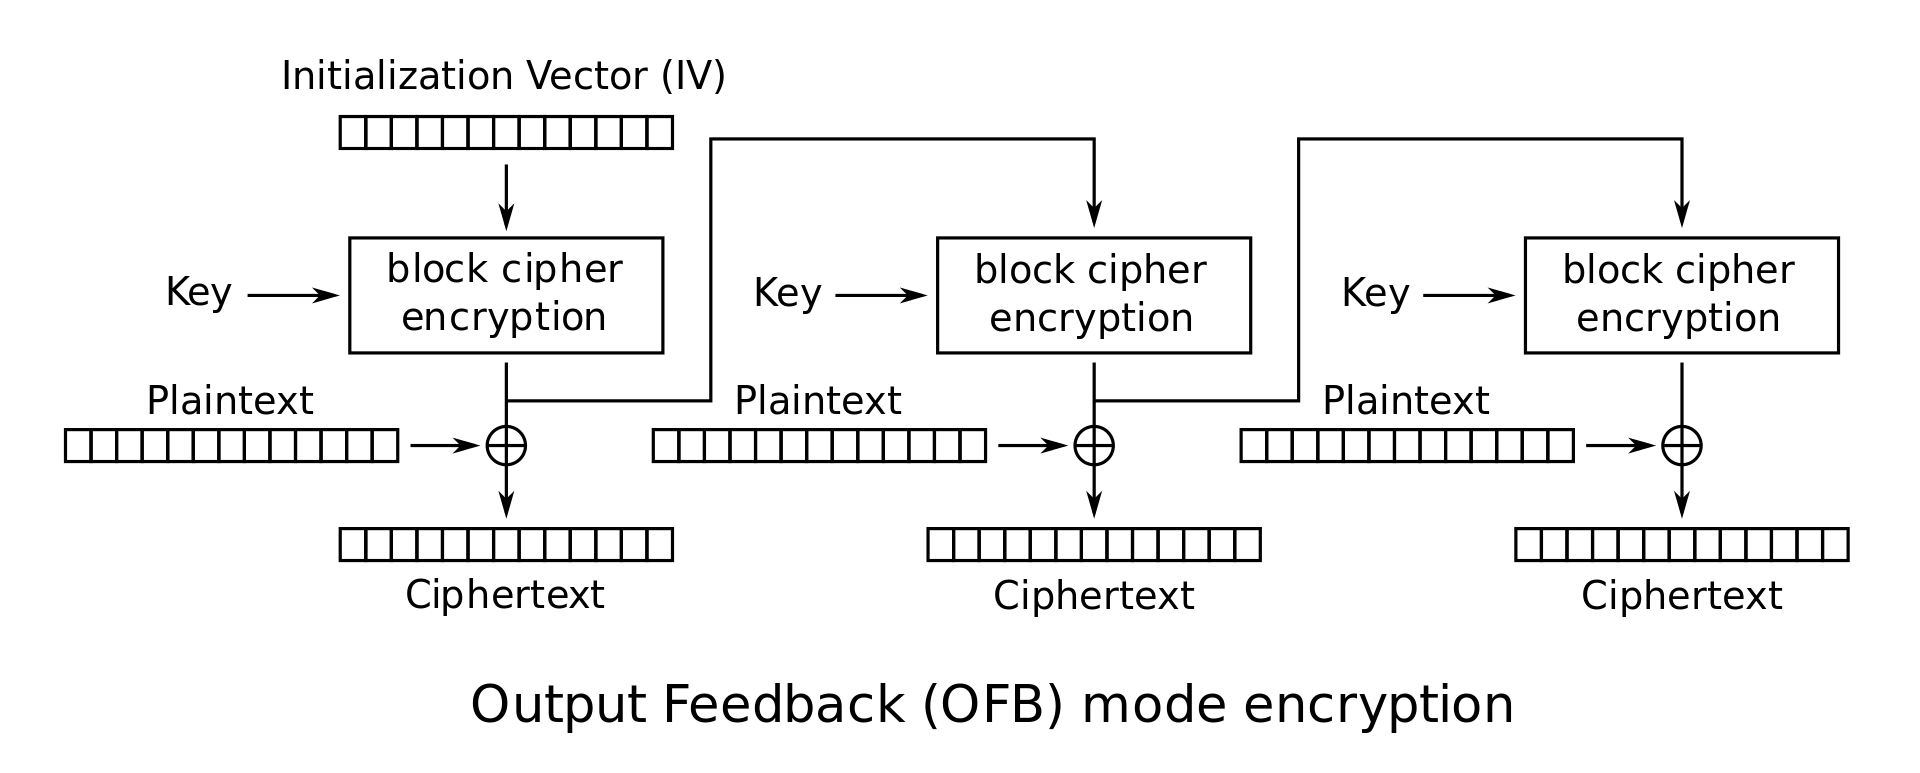
\includegraphics[width=0.5\textwidth]{figures/Ofb_encryption.png}
	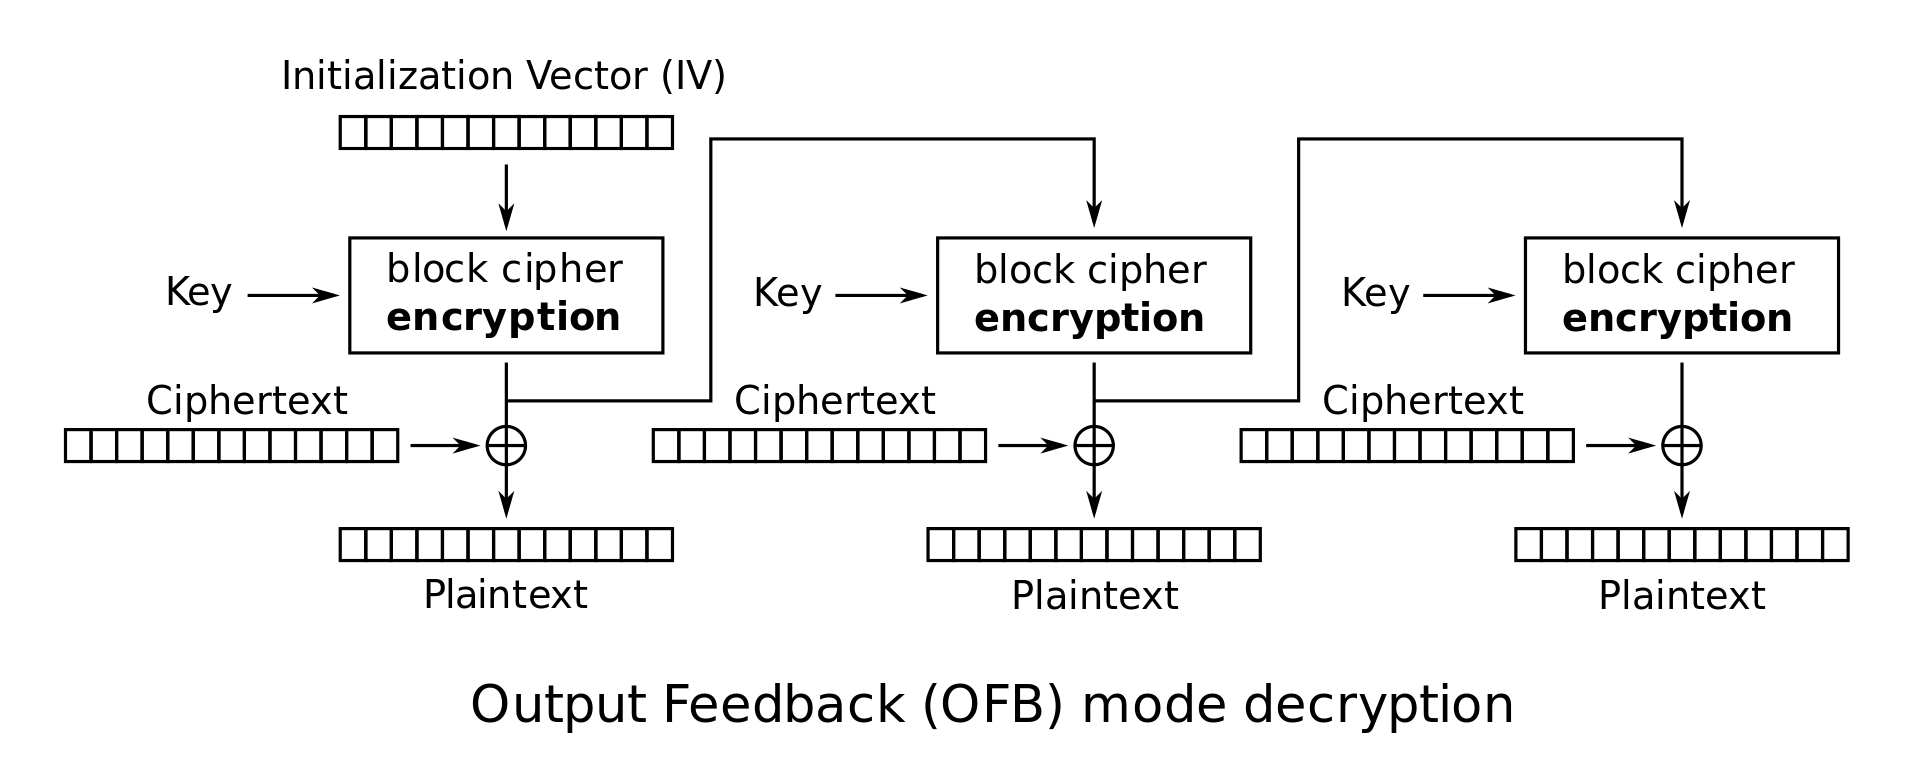
\includegraphics[width=0.5\textwidth]{figures/Ofb_decryption.png}
	\paragraph{Counter Mode (CTR)} .\\
	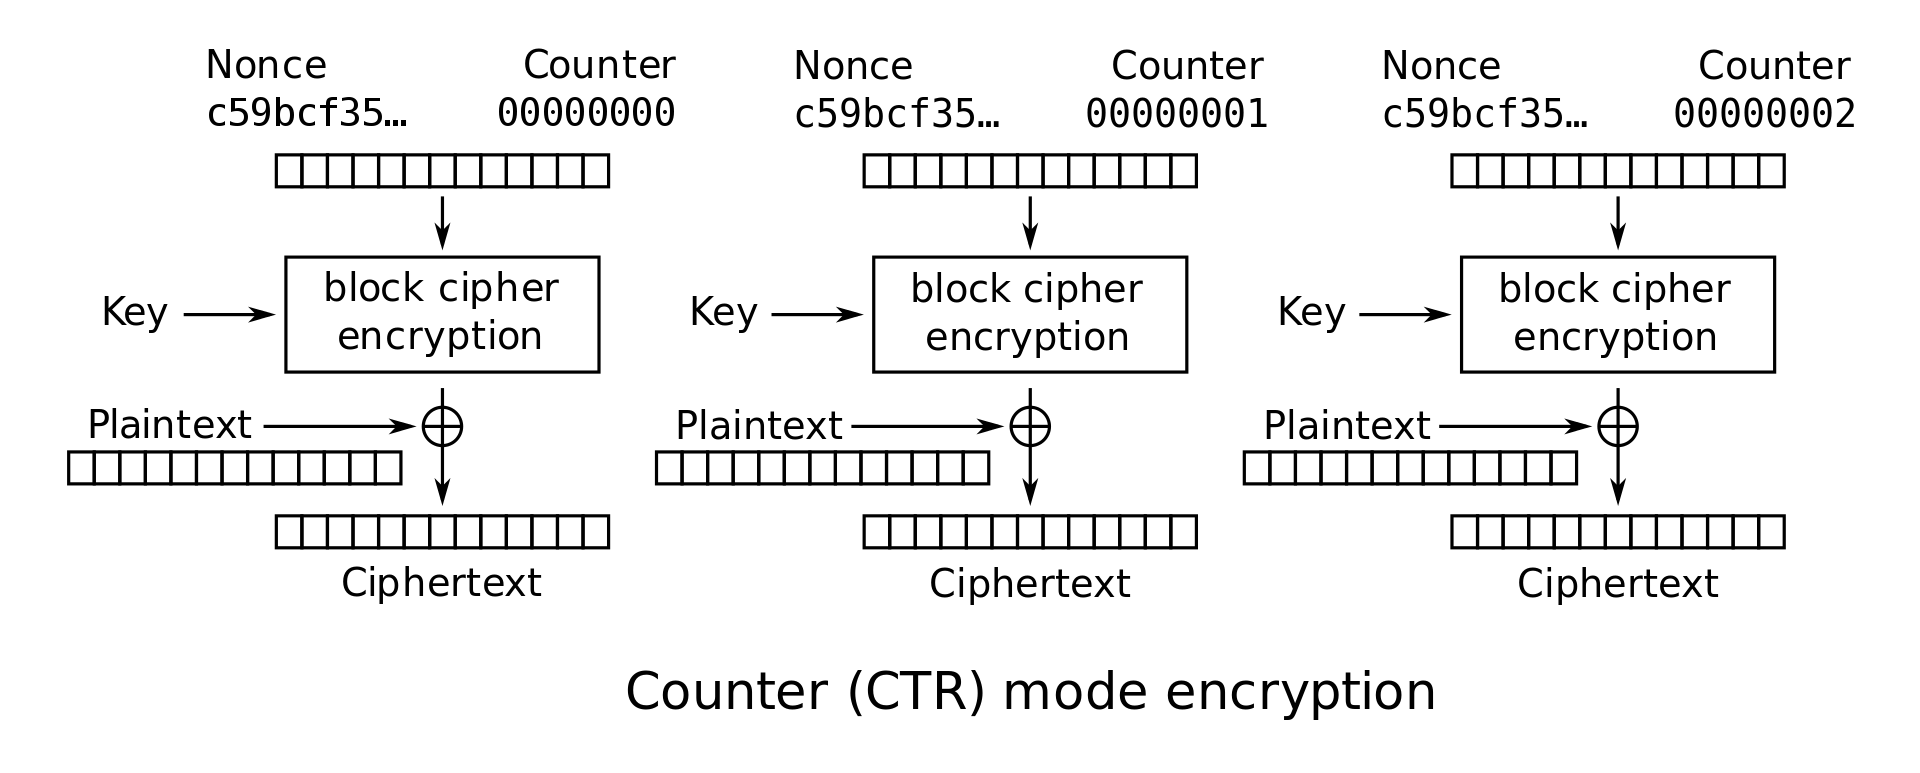
\includegraphics[width=0.5\textwidth]{figures/Ctr_encryption.png}
	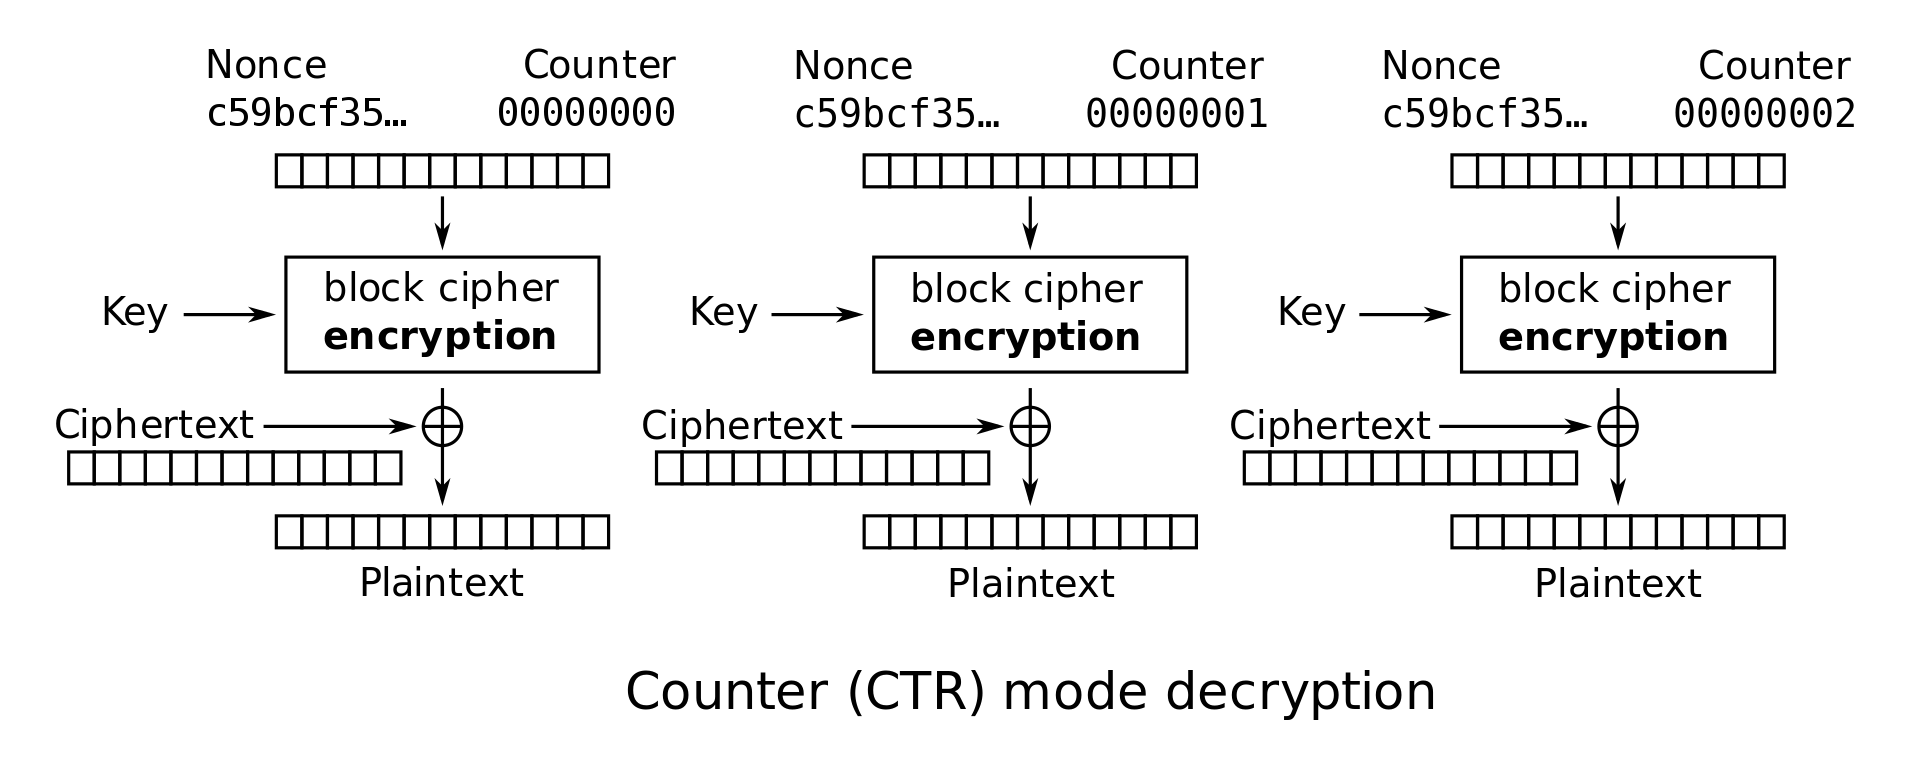
\includegraphics[width=0.5\textwidth]{figures/Ctr_decryption.png}
	
	\section{Message authentication}
	Ensure that a message is from a specified party and was not modified during transition.
	\textbf{Message authentication code (MAC) scheme} is a pair of tag ($Tag$) and verify ($Vrfy$) algorithm with $Vrfy_k(m,Tag_k(m)) = yes$ (tag is valid) for every plaintext message $m \in M$ plaintext space and key $k \in K$ key space. $Tag_k(m) = t$ generates a tag $t \in T$ set of tags. The verify algorithm just computes the tag again from the plaintext and compares the result with the given tag.\\
	$\rightarrow$ can be constructed from block ciphers (e.g. CBC-MAC) or hash functions\\
	\textbf{Replay attack} MACs do protect against the modification of the message through a third party but not against replaying an already delivered message with a valid tag again. Solution: time-stamps, sequence numbers, ...
	\textbf{Splicing attack} A CBC-MAC should be used with the message length $|m|$ as initialization vector (IV). Otherwise a splicing attack is possible:\\
	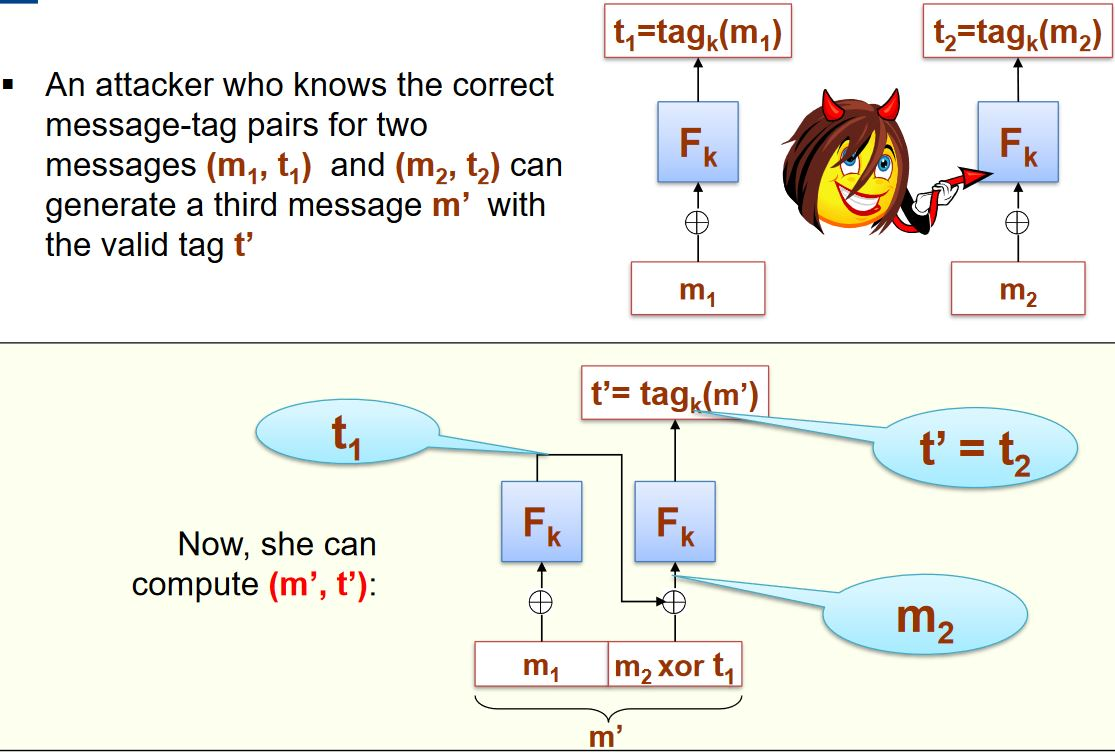
\includegraphics[width=\textwidth]{figures/splicing-attack.JPG}
	
	\subsection{Hash functions}
	Hash functions map arbitrary input to a fixed length of output. They should be collision resistant and one-way functions.(?)\\
	\textbf{Collision resistance} It's hard to find two inputs that have the same hash: $H(m) = H(m')$
	\textbf{Examples} of hash functions are MD5, SHA1, SHA2, SHA256, ...\\
	\textbf{HMAC} MAC based on a hash function: $HMAC_k(m) = H((k xor opad) || H(k xor ipad || m))$
	
	\subsection{Key distribution}
	\textbf{Key distribution center} There is an authority that all the users trust with its help it's possible to exchange session keys for direct communication. Not useful in the internet.\\
	${M}_K = Enc_{K0}(M), Tag_{K1}(Enc_{K0}(M))$ is a message $M$ that is encrypted and authenticated with key pair $K$.
	\textbf{Needham-Schroeder protocol} is a protocol for key exchange that prevents against reply and man-in-the-middle attacks (adversary can't reply the answer of the server because of the nonce, adversary can't manipulate message from Alice to Bob to change the identity who's sending the message)\\
	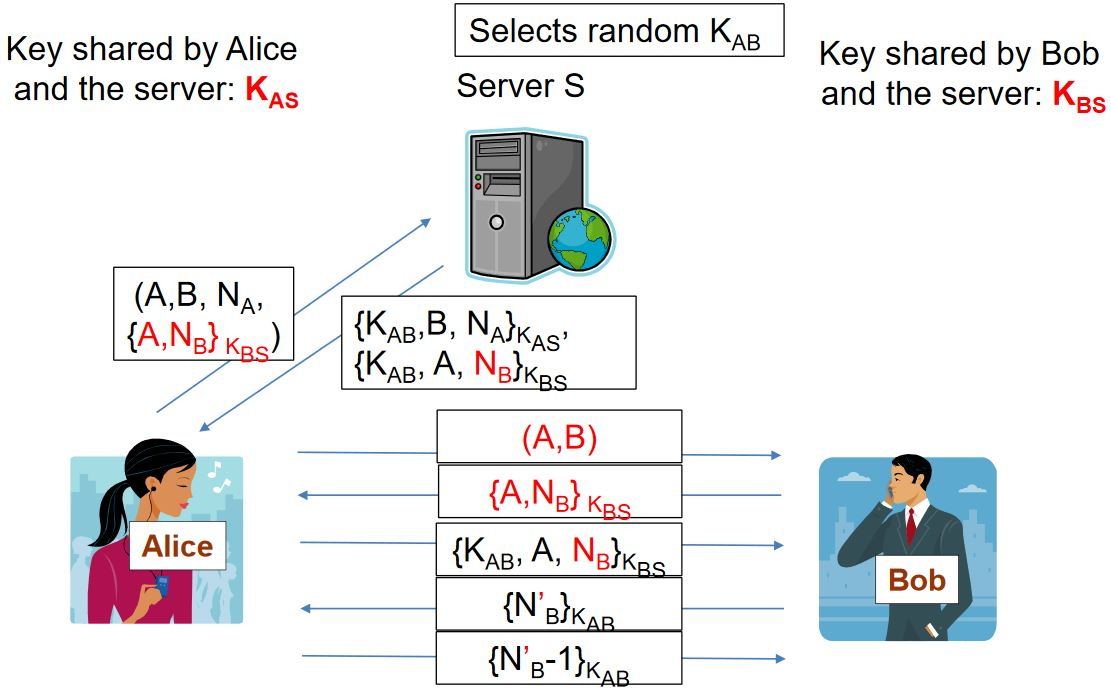
\includegraphics[width=\textwidth]{figures/needham-schroeder-protocol.JPG}\\
	\textbf{Peer-to-peer key distribution} can be achieved with public key cryptography
	
	\section{Public Key Cryptography}
	\paragraph{Encryption} Instead of using one key $k$, use a public key $pk$ for encryption and a private or secret key $sk$ for decryption.\\
	$\Rightarrow$ everyone can encrypt messages for the person who owns the private key because the encryption key is public
	\paragraph{Authentication} Use the private key to create a tag (also called signing a message) and the public key to validate the tag\\
	$\Rightarrow$ everyone can validate tags from the person who owns the private key. So signatures can be passed on and also be verified by a third party.
	\paragraph{Problems}
	\begin{itemize}
		\item how are the public keys exchanged?
		\item how to revoke keys?
	\end{itemize}
	
	\subsection{RSA algorithm}
	RSA is a trapdoor one-way function which can be inverted if a secret (the secret key) is known. The security relies on the hardness of the \textbf{factorization of large integers}.\\
	\textbf{Key generation} Generate large primes $p$, $q$ (1024 bits each is seen as secure $\rightarrow$ 2048 bit RSA)\\
	Compute $N=pq$ and $\varphi(N)=(p-1)(q-1)$, choose $e$ as co-prime to $\varphi(N)$, choose unique $d$ as inverse of $e \mod \varphi(N) \rightarrow ed = 1 \mod \varphi(N)$\\
	\textbf{Public key} = $(e,N)$, \textbf{private key} = $d$\\
	\textbf{Encryption} $c = m^e \mod N$\\
	\textbf{Decryption} $c^d \mod N = (m^e)^d \mod N = m$\\
	$\Rightarrow$ To be secure a (pseudo-)random padding is required so that the algorithm doesn't output the same ciphertext for the same plaintext.
	
	\subsection{Elgamal}
	Another public key cryptosystem which is based on the discrete logarithm hardness assumption.
	
	\subsection{Distribution of public keys}
	\textbf{Cerification Authority (CA)} signs certificates that hold the public key of a person and specify to which person it belongs. So everyone who has the public key of the CA and trusts it can verify the certificate.\\
	\textbf{Certificate Chain} CA certificates a person $P_1$ who can certificate another person $P_2$. A third person who trusts the CA and $P_1$ can now trust $P_2$. But \textbf{trust is not transitive}! CA must grant $P_1$ the right to certificate others (recommendation levels limit the length of the certification chain).\\
	\textbf{HTTPS/SSL} Root certificates that certificate a CA come with the browser and are build-in with recommendation level 1. So the browser trusts every certificate signed by the build-in CAs.
	
	\subsection{Diffie-Hellman key exchange}
	To encrypt the communication between two parties one key cryptography is used more often but the key is established using public key cryptography (for example HTTPS). This is because public key cryptography requires more computational power and is therefore slower. The Diffie-Hellman protocol is for exchanging new session keys for synchronous encryption. It relies on the hardness assumption of the difficulty of solving the \textbf{discrete logarithm problem (DLP)}.
	\begin{enumerate}
		\item choose prime $p$
		\item choose generator $g$ of $\mathbb{Z}_p^*$ (generator can compose every number in $\mathbb{Z}_p^* = x \mod p$ when multiplied with itself several times)
		\item Alice chooses random $x$ with $0 < x < p-2$ and calculates $h_1 = g^x \mod p$ and sends it to Bob
		\item Bob chooses random $y$ with $0 < y < p-2$ and calculates $h_2 = g^y \mod p$ and sends it to Alice
		\item the common key is $k = h_1^y \mod p = h_2^x \mod p = g^{xy} \mod p$
	\end{enumerate}
	$\Rightarrow$ because the logarithm in closed groups (discrete logarithm) is hard to compute this scheme is secure\\
	$\Rightarrow$ does not protect against man-in-the-middle attacks
	
	\section{Network Security}
	\textbf{Traditional network security model} trusted end nodes, unreliable network (e.g. internet)\\
	\textbf{Sniffing} Listening to network traffic and try to learn confidential information\\
	\textbf{Spoofing} Sending face messages pretending to be someone else\\
	\textbf{Man in the middle (MitM)} Manipulating message flow\\
	\textbf{Denial of Service} Attacking a service so that it is not available anymore
	
	\subsection{Internet protocol suite}
	Communication on the internet is redirected over routers which work on the network layer.\\
	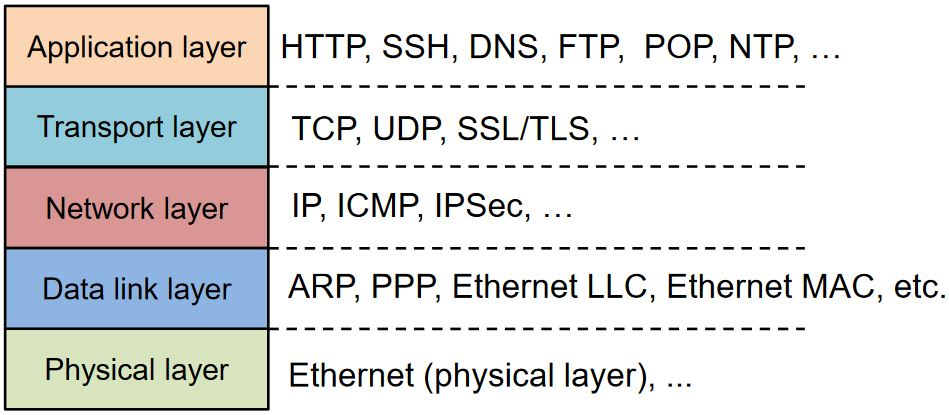
\includegraphics[width=\textwidth]{figures/internet-protocol-suite.JPG}\\
	\begin{tabular}{|l|l|l|}
		\hline 
		\textbf{Acronym} & \textbf{Full name} & \textbf{Description} \\ 
		\hline 
		HTTP & Hypertext Transfer Protocol & Request-response protocol for communication \\ 
		\hline 
		IP & Internet Protocol & Relaying packets in/between networks \\ 
		\hline 
		IPSec & IP Security Protocol & Security layer for IP \\ 
		\hline 
		TCP & Transmission Control Protocol & Connection-oriented protocol for IP networks \\ 
		\hline
		UDP & User Datagram Protocol & Exchange messages in IP network \\ 
		\hline 
		SSL/ & Secure Sockets Layer & Adds end-to-end security at transport layer \\ 
		TSL & Transport Layer Security Protocols & \\ 
		\hline 
		SSH & Secure Shell & Cryptographic layer for command shell \\ 
		\hline 
		MAC & Media Access Control & Link Layer packet delivery to hosts \\ 
		\hline 
		LLC & Logical Link Control & Flow control and error control duties \\ 
		\hline 
		DNS & Domain name system protocol & Translates domain names to IP addresses \\ 
		\hline 
		DHCP & Dynamic Host Configuration Protocol & Dynamic assignment of host configuration \\ 
		\hline 
		ICMP & Internet Control Message Protocol & Communicate errors and operational information \\ 
		\hline 
		ARP & Address resolution protocol & Maps IP to MAC address \\ 
		\hline 
	\end{tabular} 

	\subsection{Attacks}
	\paragraph{Link layer} Describes attacks on link layer protocols\\
	\textbf{MAC flooding} Switches manage a list which MAC address is connected to which port so packets for a MAC address will only be forwarded to the known port. The attacker floods the switch with new mappings so that the list runs full. If the switch now receives a packet for a MAC address it doesn't know, it is broadcasted to all ports, so the attacker can read the traffic.\\
	$\Rightarrow$ can be prevented by port security (limit mappings per port) or control network access separately\\
	\textbf{ARP attacks} ARP is a protocol to find the MAC address of a party to the given IP address within a local network. It uses request-response architecture and mapping entries get renewed even if there's no request.\\
	$\rightarrow$ Denial-of-service and man-in-the-middle possible\\
	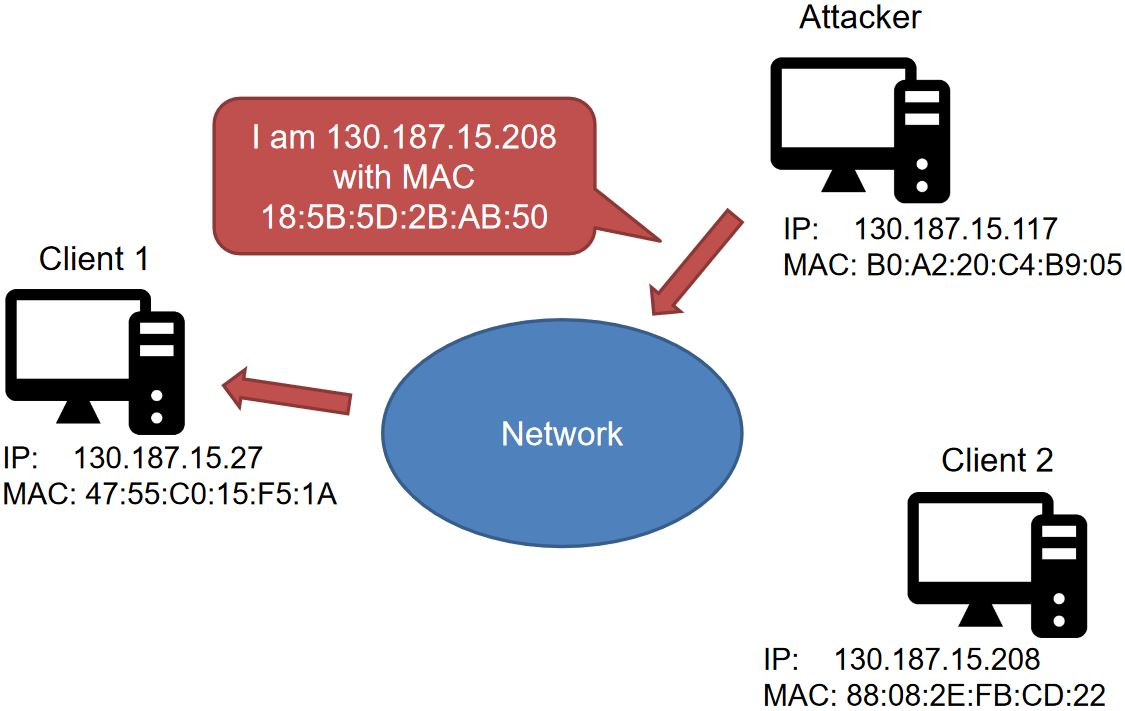
\includegraphics[width=0.5\textwidth]{figures/arp-dos1.JPG}
	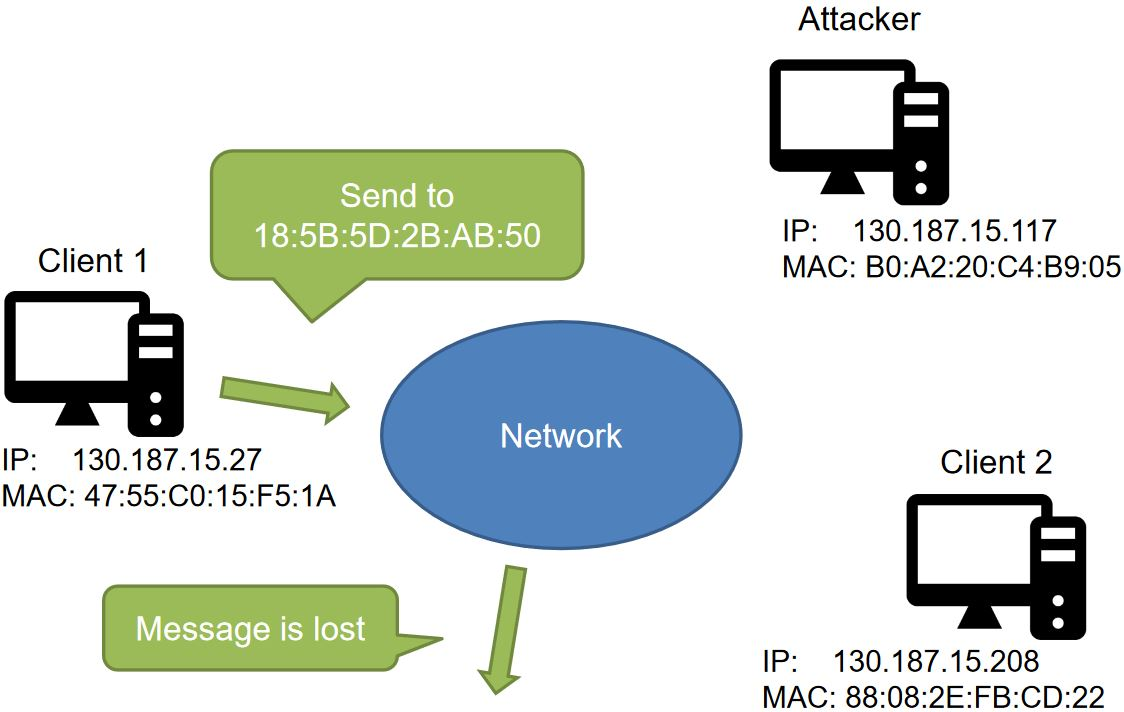
\includegraphics[width=0.5\textwidth]{figures/arp-dos2.JPG}\\
	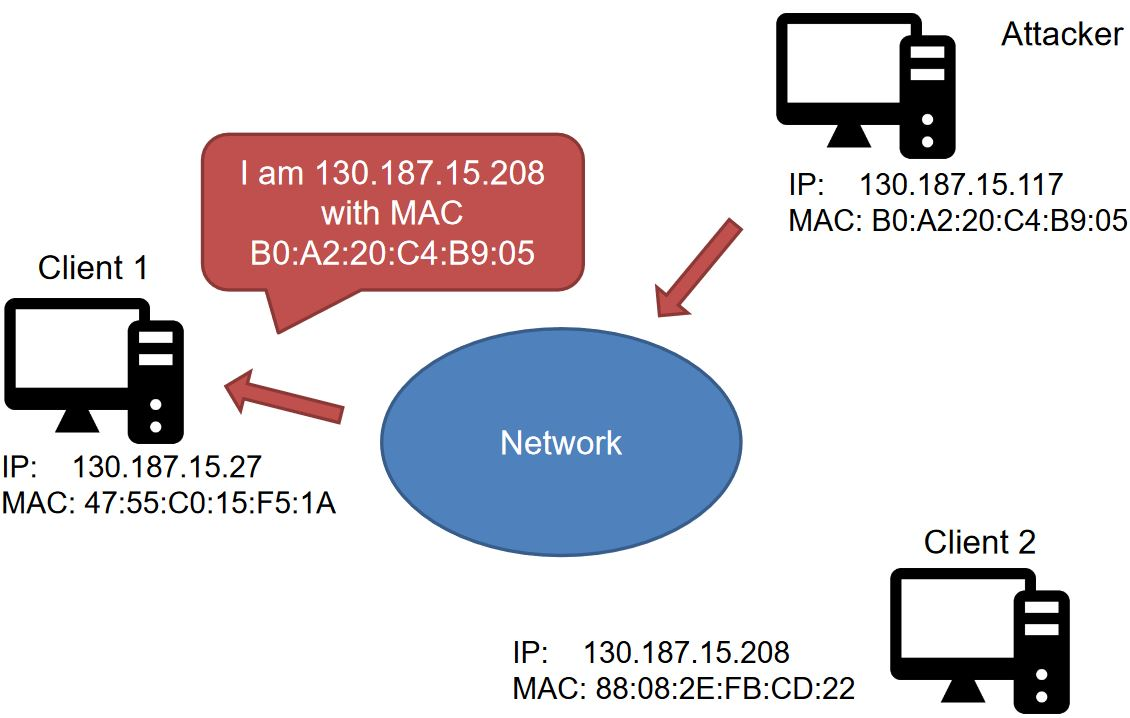
\includegraphics[width=0.33\textwidth]{figures/arp-mitm1.JPG}
	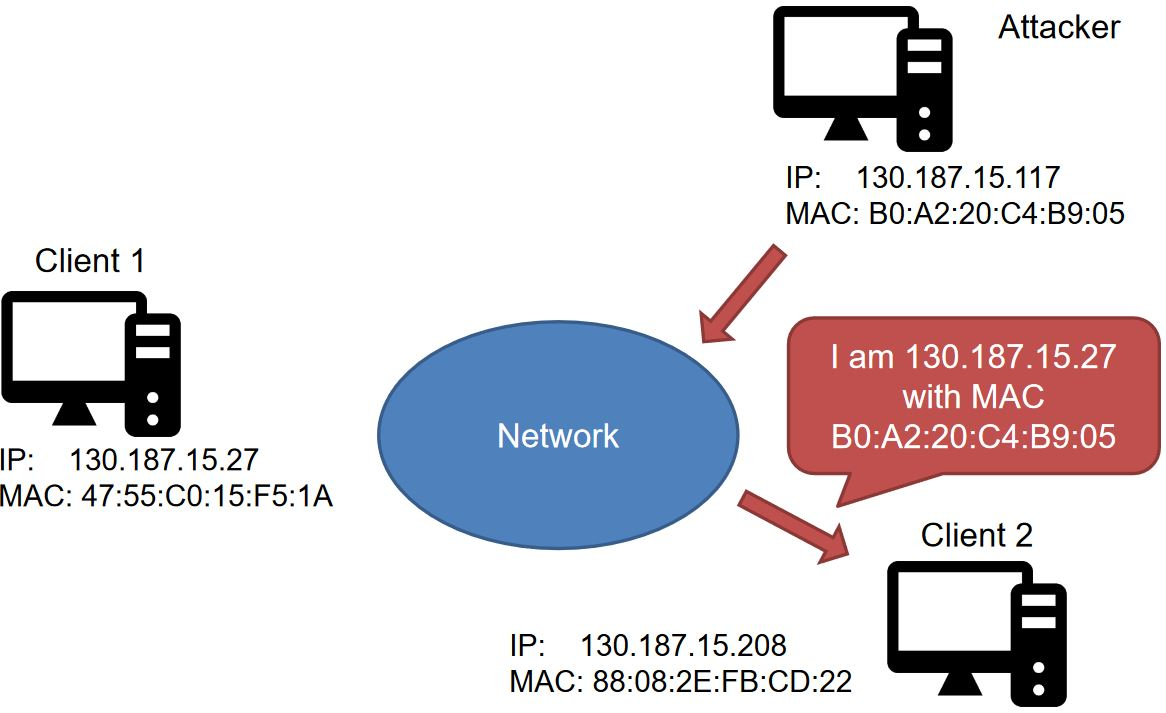
\includegraphics[width=0.33\textwidth]{figures/arp-mitm2.JPG}
	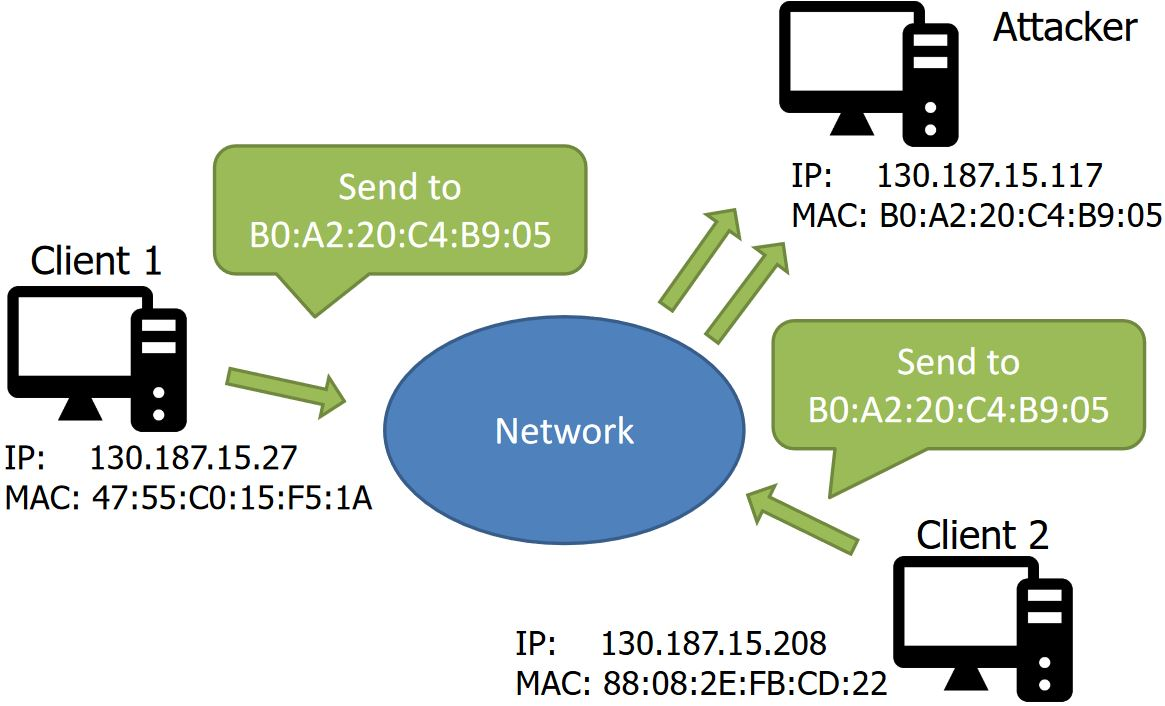
\includegraphics[width=0.33\textwidth]{figures/arp-mitm3.JPG}\\
	$\Rightarrow$ can be prevented by static ARP entries, certification and validation of responses, detect multiple IPs for single MAC
	
	\paragraph{Network layer} Describes attacks on network layer protocols\\
	\textbf{Ping flood} Send excessive amounts of ping requests to victim. This reduces the resources that can be used to answer other connections.\\
	$\Rightarrow$ Disallow pings completely, limits for ping requests (rate, size)\\
	\textbf{Smurf attack against ICMP} Send ping request with victim's IP as source address to broadcast address. Every network client will send a ping response to the victim.\\
	$\Rightarrow$ Disallow pings to broadcast addresses
	
	\paragraph{Transport layer} Describes attacks on transport layer protocols\\
	\textbf{SYN flood} Normal TCP flow: A:SYN $\rightarrow$ B:SYN-ACK $\rightarrow$ A:ACK. If an attacker A sends multiple SYN packets but not the ACK packets the server B keeps half-open connections. If its limit is reached new connections won't be accepted.\\
	$\Rightarrow$ can be prevented by dropping oldest half-open handshake, TCP Cookie Transaction (server and client support required), SYN cookie\\
	\textbf{TCP Session hijacking} Authentication of sessions often only during creation. After that an attacker could read the increasing sequence numbers from sent packets and reply to the server with the next higher sequence number to take over the session. The attacker has to be faster than the regular client.\\
	$\Rightarrow$ can be prevented by using SSL/TSL
	
	\paragraph{Application layer} Describes attacks on application layer protocols\\
	\textbf{DHCP starvation} Client asks for network configuration (e.g. IP address to use). The attacker can request multiple IP addresses to produce a denial of service when there's no free IP address left.\\
	\textbf{Rogue DHCP} Attacker claims all IP addresses. If new client requests one the attacker has to answer faster than the regular DHCP server and tell the client to take him as gateway to read his traffic $\rightarrow$ Man-in-the-middle\\
	$\Rightarrow$ can be prevented by monitoring DHCP traffic, port security to prevent attackers from using multiple MAC addresses
	\textbf{DNS amplification} DNS responses are up to 50 times larger than the requests. So by adding a victim's IP address as source an attacker can produce much traffic towards a victim (can be increased by using a botnet) $\rightarrow$ denial-of-service\\
	$\Rightarrow$ can be prevented by using DNSSEC or DNSCurve\\
	\textbf{WiFi deauthentication} An attacker can send a deauthentication frame (not encrypted) with the victim's MAC to the access point. So the victim gets disconnected.
	
	\subsection{Layer Security}
	\paragraph{Network Layer Security - IPSec} End-to-end encryption requires application layer security which is complicated to handle for the user (manage keys), for transport layer security the applications needs to be changed $\rightarrow$ network layer security can happen without the user noticing (e.g. VPN)\\
	\textbf{Modes of operation}
	\begin{itemize}
		\item Transport mode: Encrypts IP packet's payload, not the header. Used between hosts.
		\item Tunnel mode: Entire IP packet is encrypted and is payload of a surrounding new IP packet which can have different target and source addresses. Can be used between hosts, gateways or host-gateway
	\end{itemize}
	Authenticate over certificate chain, encrypt with synchronous connection key that needs to be exchanged.

	\paragraph{Transport Layer Security - SSL/TLS} Additional sublayer on top of TCP to encrypt payload. Protocols that run over TCP can run over SSL/TLS with a few changes (e.g. reserve extra port): HTTP $\rightarrow$ HTTPS, SMTP $\rightarrow$ SMTPS, ...\\
	Authenticate over certificate chain, encrypt over pre-exchanged synchronous connection key.
	
	\section{Authentication}
	Authentication for humans is not trivial because it's hard for them to remember long passphrases or keys. Usually secure channel is established then human authenticates itself.\\
	\textbf{Credentials} Claim for an identity + proof $\rightarrow$ username + password
	
	\subsection{Knowledge-based authentication}
	Identity verification via shared secret, e.g. password, pin, one-time password, questions \& answers
	\paragraph{Advantages} everyone can use it, cheap, fast, easy distribution, can be passed on, legal protection
	\paragraph{Disadvantages} user-dependent, usability vs. security, can be forgotten, observation possible (just watching, keyloggers), future security (computational power increases so must the password length/complexity)
	\paragraph{Attacks} Online cracking (brute-force) $\rightarrow$ use rate- and guess-limiting, offline cracking (e.g. password hash) $\rightarrow$ store passwords secure as hash with salt and pepper, hash cracking with rainbow tables: pre-computed table with hashes that get reduced and hashed again
	\paragraph{Entropy} Amount of missing information measured in bits. Human chosen passwords have less entropy than random ones.
	$$H = -\Sigma_{x \in passwords}(P(x) \log_2 P(x))$$
	Random passwords have entropy $H = \log_2 N$ where $N$ are all possible passwords.
	\paragraph{Challenge-Response} Authentication between client and server based on a shared secret which is not transmitted. Server generates challenge, client computes solution to challenge with shared secret and sends it to the server which checks it and returns its proof.
	
	\subsection{Ownership-based authentication}
	Identity verification via something you own, e.g. device, key files, hardware tokens (ID cards)
	\paragraph{Advantages} more entropy due to key storage, easy to revoke, depends on physical security, can be passed on like physical key
	\paragraph{Disadvantages} high costs due to hardware, easy to loose/steal, communication between hardware and reader could be eavesdropped
	
	\subsection{Inherence-based authentication}
	Identity verification via behavioral or physiological characteristics (biometrics)
	\paragraph{Advantages} can't be stolen or forgotten, easy to use
	\paragraph{Disadvantages} can't be changed when compromised, could change or become unavailable (through accidents), can't be passed on for temporary access of thirds, same login data for different services
	\paragraph{Selection of biometric parameters} universal, unique, permanent, measurable, performance, acceptable (by the population), circumvention (hard to fool the system)
	\paragraph{Examples} fingerprints (can be gained from surfaces, pictures), facial recognition (3D to prevent unlocking with photos), voice recognition, signature, DNA, iris scan, typing patterns, gait, mouse movement
	
	\subsection{Multi-factor authentication}
	Identity verification via combining multiple authentication methods $\rightarrow$ usability security trade-off\\
	For example combine passwords with face recognition, sms codes, email links, etc.
	
	\section{Software security}
	\textbf{Runtime attacks} are attacks that happen during the runtime of a program\\
	\textbf{Remote code execution} means that arbitrary code from the attacker is executed on the target system\\
	\textbf{Privilege escalation} increases the abilities that a program has to manipulate the system (e.g. normal user to admin)\\
	\textbf{Architectures} common system architectures are x86-32, x64-64, ARM\\
	\textbf{Most important registers in x86-32 architecture}\\
	\begin{tabular}{|l|l|}
		\hline 
		\textbf{Register} & \textbf{Description} \\ 
		\hline 
		EAX, EBX & general purpose registers \\ 
		ECX, EDX &  \\ 
		ESI, EDI &  \\ 
		EBP &  \\ 
		\hline 
		ESP & Stack pointer (general purpose) \\ 
		\hline 
		EIP & Instruction pointer \\ 
		\hline 
		EFLAGS & Flags for arithmetic operations (e.g. carry flag, overflow flag, ...) \\ 
		\hline 
	\end{tabular}\\
	\textbf{Endianness} defines the order of bytes in the memory
	\begin{itemize}
		\item \textbf{Big-endian format} most significant bytes first: 0xAF11 $\rightarrow$ 0x0000AF11 (32 bit) (used in IPv4, TCP, ...)
		\item \textbf{Little-endian format} least significant bytes first: 0xAF11 $\rightarrow$ 0x11AF0000 (32 bit) (used for x86-32)
	\end{itemize}
	\textbf{Memory layout}\\
	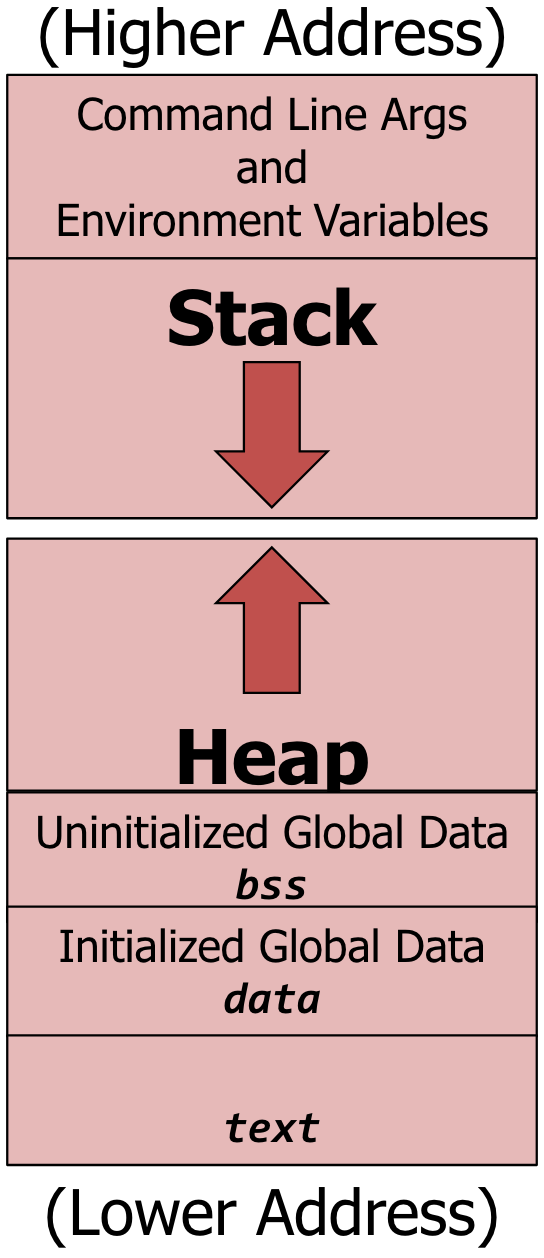
\includegraphics[width=0.2\textwidth]{figures/memory-layout.png}\\
	Stack consists out of multiple frames, one frame per function call which holds the function arguments, the return address (saved instruction pointer), saved base pointer of the calling function and local variables of the function.\\
	Manipulation of the program flow can be achieved by a buffer overflow. When the attacker enters data that is stored in a data structure without bound checking and the entered data exceeds the reserved space it will overwrite data on the stack, e.g. the return address.
	
	\subsection{Code Injection}
	The attacker tries to inject arbitrary code (often the execution of a shell) into the program flow. Not often used due to data execution prevention (DEP) which prevents code execution from writable memory.\\
	\textbf{Format string bug} Including user input in the format string of e.g. \textit{printf} is dangerous because if there are placeholder like\textit{ \%s} used and no arguments are given, this will print values from the stack. If there are more placeholders without arguments than values on the stack the program will crash $\rightarrow$ denial-of-service
	
	\subsection{Code reuse} The attacker tries to manipulate the program flow so that existing code is executed in a different order, e.g. call security-critical functions in shared libraries (libc is often linked to most C programs). To achieve arbitrary code execution the attacker can try to use return-oriented programming.
	
	\paragraph{Return-oriented programming (ROP)} Combine small instruction sequences (e.g. of libc) with return statements at the end to gadgets that perform a particular operation (e.g. load, store, xor, ...). By jumping from one gadget to the other (performing buffer overflow attacks to set the return address) arbitrary computations are possible. It's easy to achieve a Turing-complete language because only a few gadgets/commands are required: conditional jump, store, load\\
	\textbf{Defense strategies}\\
	\textbf{Shadow stack} is a copy of the original stack to validate whether a return instruction targets its original caller\\
	\textbf{Remove unintended return instructions} to minimize the gadget space\\
	\textbf{Behavioral-based heuristics} check the number of instructions executed between return instructions $\rightarrow$ affords computational power
	
	\paragraph{Jump-oriented programming (JOP)} This tries to manipulate the jump address for indirect jumps or call instructions instead of manipulating the return address on the stack. This requires a sequence of \textbf{u}pdating the global state, \textbf{l}oading the address of the next instruction, \textbf{b}ranch to the address loaded $\rightarrow$ a so called ULB-sequence which doesn't occur very often. That's why its reused as a "trampoline sequence" which is called after every gadget.\\
	This can also achieve a Turing-complete language and bypasses the defense strategies for ROP.\\
	\textbf{Defense strategies}\\
	\textbf{Stack canaries/stack cookies} Insert random "canary" value next to sensitive information (e.g. end of buffer) on the stack. With a buffer overflow the attacker would overwrite the canary value which should then be checked before a jump or return instruction. If the canary was overwritten the program should terminate.\\
	\textbf{Control-flow integrity (CFI)} Build a graph of the program flow and check it when the program flow is redirected (jump, call, return). This affords a lot of computational power, still hot research topic.\\
	\textbf{Software diversity} Compile program $N$ times with a different memory layout each time so that an exploit can only affect one of them.\\
	$\Rightarrow$ Unpractical for software distribution because usually software binaries are downloaded so everyone has the same memory layout.\\
	\textbf{Address space layout randomization (ASLR)} randomizes the base address of code/data segments at startup. Can be compromised using brute-force if processes are cloned with the same address space layout (e.g. Apache Webserver)\\
	\\
	\begin{tabular}{|l|l|}
		\hline 
		\textbf{randomization} & \textbf{control-flow integrity} \\ 
		\hline 
		+ low performance overhead & - high performance overhead \\ 
		+ scales well to complex software & - hard to integrate in complex software \\ 
		- high entropy required & + strong security guarantees \\ 
		- memory disclosure hard to prevent & - tradeoff: performance \& security \\ 
		\hline 
	\end{tabular}

	\section{Platform security}
	Platform security takes care of attackers within the computer system. Core security mechanisms:
	\begin{itemize}
		\item \textbf{Isolation}: separate systems can only interact over pre-defined interfaces
		\item \textbf{Access Control (AC)}: control access to system resources (files, memory areas, external devices, CPU, ...) $\rightarrow$ limits access between subjects and objects, traditionally authentication + authorization
	\end{itemize}
	\textbf{User} of a computer system can be a human being or an agent, both are equal in terms of platform security and have an account or profile.\\
	\textbf{Subject} is an active entity such as a running process.\\
	\textbf{Object} is a passive entity such as a file or a database record.\\
	\textbf{Monolithic design} means that a system has several inputs and outputs but the internals of the system can freely communicate between each other. $\rightarrow$ once an attacker is in the system he has access to everything.\\
	\textbf{Component design} means that the system consists out of several components that can be seen as individual subsystems with dedicated in- and output interfaces. $\rightarrow$ It's harder for the attacker to compromise the system because he has to infiltrate every component.\\
	\textbf{Trusted computing base (TCB)} includes all systems that need to be trusted to implement system-critical functionality (e.g. access control)\\
	\textbf{Security design principles}
	\begin{itemize}
		\item Economy of mechanism: keep the design simple and small
		\item Complete mediation: check access rights for every access
		\item Open design: no security by obscurity, discuss design openly
		\item Least-common mechanism: minimize the amount of common components to more than one user
		\item Fail-safe defaults: refuse access if not specified differently
		\item Separation of privilege: different access rights for different resources (e.g. network and file system)
		\item Least privileges: every system user should only obtain the minimal set of required privileges
		\item Privacy considerations: every information should be considered as private and only passed on if necessary
		\item Psychological acceptance: usability of security systems is important to be aware of, otherwise users won't use it
	\end{itemize}

	\subsection{Access control models}
	\paragraph{Discretionary access control (DAC)} Users declare who has access to their data. The owner of data gives the access rights e.g. by creating passwords for directories of files (problem of revocation). $\rightarrow$ can be enhanced by access control lists or matrices (ACL, ACM) which lists the abilities for every subject to perform actions on any object.
	
	\paragraph{Mandatory access control (MAC)} Access is controlled with rules set by the system administrator, e.g. DRM (music purchased can be played but not shared). The access privileges can't be passed on.
	
	\paragraph{Role-based access control (RBAC)} Users are mapped to roles which have specific access rights. Users/subjects are collected in groups, access rights on objects are collected in roles. Roles can form hierarchies.
	
	\paragraph{Chinese Wall model} Information/objects that are in a conflict should not be accessed by the same subject (e.g. tax information about competing clients) so if a subject S accesses one of the objects it won't be able to access the conflicting object (S falls on one side of the wall).\\
	$\Rightarrow$ separation of duty policies are stateful and need to remember all past events
	
	\paragraph{Attribute-based access control} Access is granted or denied depending on attributes/properties of the subject (e.g. location, age, etc.)
	
	\subsection{Process isolation in operating systems}
	Processes need to be isolated because the physical memory is a shared resource that needs protection (e.g. process should not overwrite other processes' memory). This is achieved by memory virtualization. Every process believes it owns the hole memory and can write to all addresses. The OS translates access to virtual memory addresses to physical ones.To modify the address translation table the CPU must be in kernel mode (user mode and kernel mode are implemented in hardware).\\
	\textbf{Switching user mode $\rightarrow$ kernel mode} to run a user program
	\begin{enumerate}
		\item create process and initialize address space
		\item load the program to the memory
		\item initialize translation table
		\item set hardware pointer to the translation table
		\item set CPU to user mode
		\item jump to program entry
	\end{enumerate}
	\textbf{Switching kernel mode $\rightarrow$ user mode} for system calls (program asks os to do something for it), hardware interrupts, program exceptions
	\begin{enumerate}
		\item set CPU to kernel mode
		\item save program counter
		\item jump to handler in os kernel
		\item the handler saves old register values
	\end{enumerate}

	\subsection{Access control in operating systems}
	\paragraph{AC in UNIX/LINUX} Users have username and user id (0 = root = superuser), are collected in groups that have names and ids, too. The account information is stored in \textit{/etc/passwd} in this format:
	\begin{center}
		\textit{username:password (as hash):UID:GID (of primary group):name:homedir:shell}
	\end{center}
	and the group information is stored in \textit{/etc/group} in this format:
	\begin{center}
		\textit{groupname:password:GID:list of users}
	\end{center}
	\textbf{Subjects} are processes that have ids (PID) and can create new processes. They have a real UID/GID e.g. from the logged-in user and an effective UID/GID from the file being executed or the parent process.\\
	\textbf{Objects} are files, directories or devices that are organized in a tree-like file system. They all store information about the owner user and group and the permissions.\\
	\textbf{Permissions} for the objects are grouped for the owner, the owning group and other users (r = read access, w = write access, x = executable, s = executes with the effective UID or GID of the owning user or group). Only processes running as root can listen to TCP or UDP ports 0-1023.\\
	Default permissions for files: 666, for executables: 777. Umask restricts them.
	
	\paragraph{AC in Windows} Principals are users, machines, groups, etc. They have a unique security identifier (SID). Users are stored either locally on a machine or on a server that acts as domain controller (DC) in an active directory (AD)\\
	\textbf{Subjects} are processes or threads that act for a principal. They hold access tokens that are managed in a list to map them to objects access rights.\\
	\textbf{Objects} are files, registry keys, printers, etc. They have a security descriptor which holds the discretionary access control list (DACL) that can be modified by its owner and holds SIDs with corresponding access rights (access control entities = ACEs).\\
	\textbf{Login} winlogon.exe takes credentials, Local Security Authority (LSA, lsass.exe) verifies them. The logon process starts a shell (explorer.exe) running as the user (= principal) in a new login session. All processes of a login session get destroyed during logout.\\
	\textbf{Inheritance} ACEs are inherited from parent containers. To accelerate the permission check they are cached in child objects which results in a long waiting time when the permissions of a high level container are changed (because they are copied to every child).\\
	\textbf{User account control (UAC)} Users have two tokens, one with restricted privileges and one with admin privileges. UAC pops up when a process wants to elevate to gain admin privileges.
	
	\paragraph{AC on mobile systems} Android, iOS\\
	\textbf{Subjects} are apps that get permissions to access objects when needed. Apps are isolated and can access only the internet and their own data by default. There's no possibility to communicate between apps through file storage.\\
	\textbf{Objects} are phone features and services such as location, sms, camera, etc.
	
	\end{document}
